% Options for packages loaded elsewhere
\PassOptionsToPackage{unicode}{hyperref}
\PassOptionsToPackage{hyphens}{url}
\PassOptionsToPackage{dvipsnames,svgnames,x11names}{xcolor}
%
\documentclass[
  letterpaper,
  DIV=11,
  numbers=noendperiod]{scrartcl}

\usepackage{amsmath,amssymb}
\usepackage{lmodern}
\usepackage{iftex}
\ifPDFTeX
  \usepackage[T1]{fontenc}
  \usepackage[utf8]{inputenc}
  \usepackage{textcomp} % provide euro and other symbols
\else % if luatex or xetex
  \usepackage{unicode-math}
  \defaultfontfeatures{Scale=MatchLowercase}
  \defaultfontfeatures[\rmfamily]{Ligatures=TeX,Scale=1}
\fi
% Use upquote if available, for straight quotes in verbatim environments
\IfFileExists{upquote.sty}{\usepackage{upquote}}{}
\IfFileExists{microtype.sty}{% use microtype if available
  \usepackage[]{microtype}
  \UseMicrotypeSet[protrusion]{basicmath} % disable protrusion for tt fonts
}{}
\makeatletter
\@ifundefined{KOMAClassName}{% if non-KOMA class
  \IfFileExists{parskip.sty}{%
    \usepackage{parskip}
  }{% else
    \setlength{\parindent}{0pt}
    \setlength{\parskip}{6pt plus 2pt minus 1pt}}
}{% if KOMA class
  \KOMAoptions{parskip=half}}
\makeatother
\usepackage{xcolor}
\setlength{\emergencystretch}{3em} % prevent overfull lines
\setcounter{secnumdepth}{-\maxdimen} % remove section numbering
% Make \paragraph and \subparagraph free-standing
\ifx\paragraph\undefined\else
  \let\oldparagraph\paragraph
  \renewcommand{\paragraph}[1]{\oldparagraph{#1}\mbox{}}
\fi
\ifx\subparagraph\undefined\else
  \let\oldsubparagraph\subparagraph
  \renewcommand{\subparagraph}[1]{\oldsubparagraph{#1}\mbox{}}
\fi


\providecommand{\tightlist}{%
  \setlength{\itemsep}{0pt}\setlength{\parskip}{0pt}}\usepackage{longtable,booktabs,array}
\usepackage{calc} % for calculating minipage widths
% Correct order of tables after \paragraph or \subparagraph
\usepackage{etoolbox}
\makeatletter
\patchcmd\longtable{\par}{\if@noskipsec\mbox{}\fi\par}{}{}
\makeatother
% Allow footnotes in longtable head/foot
\IfFileExists{footnotehyper.sty}{\usepackage{footnotehyper}}{\usepackage{footnote}}
\makesavenoteenv{longtable}
\usepackage{graphicx}
\makeatletter
\def\maxwidth{\ifdim\Gin@nat@width>\linewidth\linewidth\else\Gin@nat@width\fi}
\def\maxheight{\ifdim\Gin@nat@height>\textheight\textheight\else\Gin@nat@height\fi}
\makeatother
% Scale images if necessary, so that they will not overflow the page
% margins by default, and it is still possible to overwrite the defaults
% using explicit options in \includegraphics[width, height, ...]{}
\setkeys{Gin}{width=\maxwidth,height=\maxheight,keepaspectratio}
% Set default figure placement to htbp
\makeatletter
\def\fps@figure{htbp}
\makeatother

\KOMAoption{captions}{tableheading}
\makeatletter
\makeatother
\makeatletter
\makeatother
\makeatletter
\@ifpackageloaded{caption}{}{\usepackage{caption}}
\AtBeginDocument{%
\ifdefined\contentsname
  \renewcommand*\contentsname{Table of contents}
\else
  \newcommand\contentsname{Table of contents}
\fi
\ifdefined\listfigurename
  \renewcommand*\listfigurename{List of Figures}
\else
  \newcommand\listfigurename{List of Figures}
\fi
\ifdefined\listtablename
  \renewcommand*\listtablename{List of Tables}
\else
  \newcommand\listtablename{List of Tables}
\fi
\ifdefined\figurename
  \renewcommand*\figurename{Figure}
\else
  \newcommand\figurename{Figure}
\fi
\ifdefined\tablename
  \renewcommand*\tablename{Table}
\else
  \newcommand\tablename{Table}
\fi
}
\@ifpackageloaded{float}{}{\usepackage{float}}
\floatstyle{ruled}
\@ifundefined{c@chapter}{\newfloat{codelisting}{h}{lop}}{\newfloat{codelisting}{h}{lop}[chapter]}
\floatname{codelisting}{Listing}
\newcommand*\listoflistings{\listof{codelisting}{List of Listings}}
\makeatother
\makeatletter
\@ifpackageloaded{caption}{}{\usepackage{caption}}
\@ifpackageloaded{subcaption}{}{\usepackage{subcaption}}
\makeatother
\makeatletter
\@ifpackageloaded{tcolorbox}{}{\usepackage[many]{tcolorbox}}
\makeatother
\makeatletter
\@ifundefined{shadecolor}{\definecolor{shadecolor}{rgb}{.97, .97, .97}}
\makeatother
\makeatletter
\makeatother
\ifLuaTeX
  \usepackage{selnolig}  % disable illegal ligatures
\fi
\IfFileExists{bookmark.sty}{\usepackage{bookmark}}{\usepackage{hyperref}}
\IfFileExists{xurl.sty}{\usepackage{xurl}}{} % add URL line breaks if available
\urlstyle{same} % disable monospaced font for URLs
\hypersetup{
  pdftitle={ABC Bank Ltd.},
  pdfauthor={amol},
  colorlinks=true,
  linkcolor={blue},
  filecolor={Maroon},
  citecolor={Blue},
  urlcolor={Blue},
  pdfcreator={LaTeX via pandoc}}

\title{ABC Bank Ltd.}
\usepackage{etoolbox}
\makeatletter
\providecommand{\subtitle}[1]{% add subtitle to \maketitle
  \apptocmd{\@title}{\par {\large #1 \par}}{}{}
}
\makeatother
\subtitle{Cognext model}
\author{amol}
\date{22-08-2022}

\begin{document}
\maketitle
\ifdefined\Shaded\renewenvironment{Shaded}{\begin{tcolorbox}[interior hidden, sharp corners, breakable, enhanced, frame hidden, boxrule=0pt, borderline west={3pt}{0pt}{shadecolor}]}{\end{tcolorbox}}\fi

\renewcommand*\contentsname{Table of contents}
{
\hypersetup{linkcolor=}
\setcounter{tocdepth}{3}
\tableofcontents
}
\hypertarget{executive-summary} on validation dataset and \textbf{74.98\%} on
Out-of-Sample (OOS) test dataset.

\hypertarget{model-performance-summary}{%
\subsection{MODEL PERFORMANCE SUMMARY}\label{model-performance-summary}}

\begin{longtable}[]{@{}
  >{\raggedright\arraybackslash}p{(\columnwidth - 4\tabcolsep) * \real{0.5417}}
  >{\raggedright\arraybackslash}p{(\columnwidth - 4\tabcolsep) * \real{0.2083}}
  >{\raggedright\arraybackslash}p{(\columnwidth - 4\tabcolsep) * \real{0.2500}}@{}}
\toprule()
\begin{minipage}[b]{\linewidth}\raggedright
Dataset
\end{minipage} & \begin{minipage}[b]{\linewidth}\raggedright
Size
\end{minipage} & \begin{minipage}[b]{\linewidth}\raggedright
Auto
\end{minipage} \\
\midrule()
\endhead
Validation & 1920 & 75.84\% \\
OSS Test & 1990 & 74.98\% \\
\bottomrule()
\end{longtable}

\hypertarget{dataset}{%
\subsection{DATASET}\label{dataset}}

Following dataset were used for model training, tuning and OOS
performance estimation:

\begin{longtable}[]{@{}
  >{\raggedright\arraybackslash}p{(\columnwidth - 6\tabcolsep) * \real{0.2200}}
  >{\raggedright\arraybackslash}p{(\columnwidth - 6\tabcolsep) * \real{0.2800}}
  >{\raggedright\arraybackslash}p{(\columnwidth - 6\tabcolsep) * \real{0.2600}}
  >{\raggedright\arraybackslash}p{(\columnwidth - 6\tabcolsep) * \real{0.2400}}@{}}
\toprule()
\begin{minipage}[b]{\linewidth}\raggedright
Dataset
\end{minipage} & \begin{minipage}[b]{\linewidth}\raggedright
Size
\end{minipage} & \begin{minipage}[b]{\linewidth}\raggedright
Features
\end{minipage} & \begin{minipage}[b]{\linewidth}\raggedright
Purpose
\end{minipage} \\
\midrule()
\endhead
Train & 1690 & 70 & Model training \\
Validation & 1920 & 70 & Hyperparameter tuning \\
OSS Test & 1990 & 70 & OOS performance estimation \\
\bottomrule()
\end{longtable}

\hypertarget{eda}{%
\subsection{EDA}\label{eda}}

Following is a summary of input data. Refer Annexure-1 for detailed EDA.

\begin{figure}

{\centering 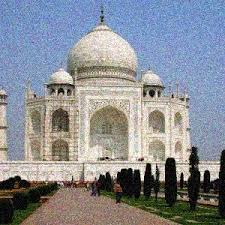
\includegraphics{Images/images.jpeg}

}

\caption{Image}

\end{figure}

\hypertarget{methodology-overview}{%
\subsection{Methodology Overview}\label{methodology-overview}}

XGBoost XGBoost is a fast and efficient implementation of gradient
boosting algorithm. Gradient boosting is a machine learning technique
for regression and classification problems, which produces a prediction
model in the form of an ensemble of weak prediction models, typically
decision trees.

\begin{longtable}[]{@{}
  >{\raggedright\arraybackslash}p{(\columnwidth - 4\tabcolsep) * \real{0.1806}}
  >{\raggedright\arraybackslash}p{(\columnwidth - 4\tabcolsep) * \real{0.1250}}
  >{\raggedright\arraybackslash}p{(\columnwidth - 4\tabcolsep) * \real{0.1250}}@{}}
\toprule()
\begin{minipage}[b]{\linewidth}\raggedright
Dataset
\end{minipage} & \begin{minipage}[b]{\linewidth}\raggedright
Size
\end{minipage} & \begin{minipage}[b]{\linewidth}\raggedright
Auto
\end{minipage} \\
\midrule()
\endhead
Validation & 1920 & 75.84\% \\
OSS Test & 1990 & 74.98\% \\
\bottomrule()
\end{longtable}

Following is a summary of steps performed to train the model:
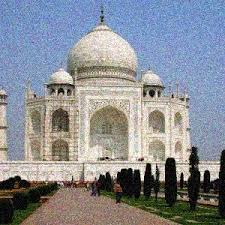
\includegraphics{Images/images.jpeg}

\hypertarget{data-preparation}{%
\subsubsection{Data Preparation}\label{data-preparation}}

The dataset is randomly split into train, validation and holdout test
datasets. Train data is used for model fitting. Validation dataset is
used for model tuning i.e.~finding the optimal combination of
hyperparameters that provide the best fit on a given dataset. Holdout
test dataset is used to arrive at an unbiased estimate of OOS
performance of the model.

\hypertarget{feature-transformation}{%
\subsubsection{Feature Transformation}\label{feature-transformation}}

Typically all features are converted into numeric features. This is a
mandatory transformation for many algorithms such as XGBoost.

\hypertarget{model-tuning}{%
\subsubsection{Model Tuning}\label{model-tuning}}

Various models are fitted to the train dataset with multiple combination
of hyperparameters (HP). These HP typically control model capacity
(large capacity models will provide better fit on train data but may
fail to generalize to OOS dataset), model complexity (typically models
with larger capacity are also more complex) and model generalization (to
prevent overfitting to train data).

\hypertarget{model-performance-evaluation}{%
\subsubsection{Model Performance
Evaluation}\label{model-performance-evaluation}}

Performance of trained models is compared on validation dataset using
different statistics. Final HP combination and the resultant final model
is selected on basis of performance on the validation dataset.

\hypertarget{model-stability}{%
\subsubsection{Model Stability}\label{model-stability}}

Model stability is checked by detecting drift/shift in features between
train, validation and test dataset. This is done by computing Stability
Index at model and individual feature level to identify if model is
stable or not.

\hypertarget{model-details}{%
\subsection{Model Details}\label{model-details}}

Detailed Information regarding model.

\hypertarget{model-hyperparameters}{%
\subsubsection{Model Hyperparameters}\label{model-hyperparameters}}

Following is a summary of key model hyperparameters:

\begin{longtable}[]{@{}
  >{\raggedright\arraybackslash}p{(\columnwidth - 4\tabcolsep) * \real{0.1806}}
  >{\raggedright\arraybackslash}p{(\columnwidth - 4\tabcolsep) * \real{0.1250}}
  >{\raggedright\arraybackslash}p{(\columnwidth - 4\tabcolsep) * \real{0.1250}}@{}}
\toprule()
\begin{minipage}[b]{\linewidth}\raggedright
Dataset
\end{minipage} & \begin{minipage}[b]{\linewidth}\raggedright
Size
\end{minipage} & \begin{minipage}[b]{\linewidth}\raggedright
Auto
\end{minipage} \\
\midrule()
\endhead
Validation & 1920 & 75.84\% \\
OSS Test & 1990 & 74.98\% \\
\bottomrule()
\end{longtable}

`+--------+------------+-------+\n\textbar{} Name \textbar{} LastName
\textbar{} Age \textbar{}\n+========+============+=======+\n\textbar{}
Name \textbar{} LastName \textbar{} Age
\textbar{}\n+--------+------------+-------+\n\textbar{} Juan \textbar{}
Lopez \textbar{} 22
\textbar{}\n+--------+------------+-------+\n\textbar{} Luisa \textbar{}
Perez \textbar{} 24
\textbar{}\n+--------+------------+-------+\n\textbar{} Ana \textbar{}
Sanchez \textbar{} 23 \textbar{}\n+--------+------------+-------+'
\#\#\# Important Features Following is a list of important features for
the model: \textbar{} Dataset \textbar{} Size \textbar{} Auto \textbar{}
\textbar-------------\textbar-----\textbar------\textbar{} \textbar{}
Validation \textbar{} 1920 \textbar{} 75.84\% \textbar{} \textbar{} OSS
Test \textbar{} 1990 \textbar{} 74.98\% \textbar{}

\begin{figure}

{\centering 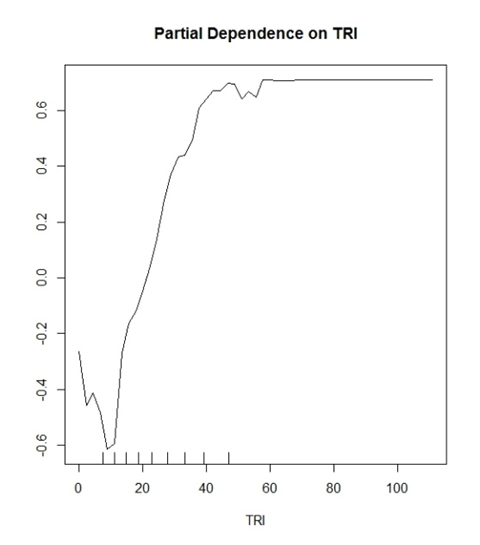
\includegraphics{Images/pdg.png}

}

\caption{Partial Dependance Graph}

\end{figure}

\hypertarget{model-performance}{%
\subsubsection{Model Performance}\label{model-performance}}

Following are the model performance statistics on validation and OOS
test dataset: \textbf{Validation dataset}

\begin{figure}

{\centering 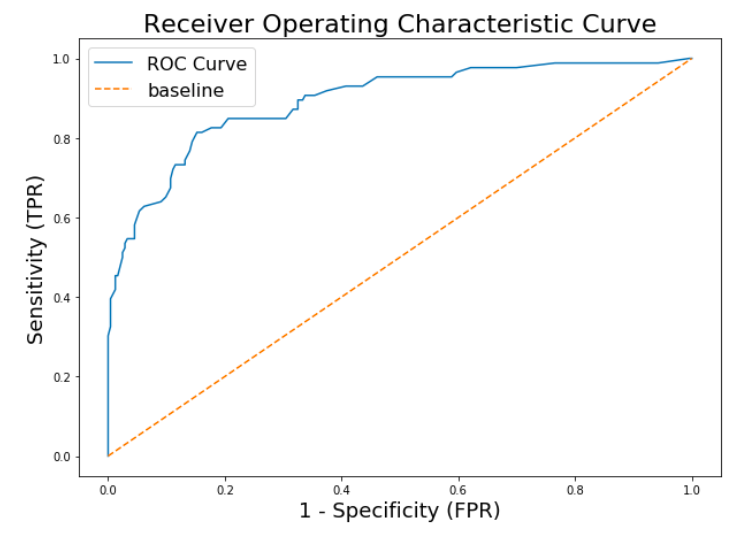
\includegraphics{Images/roc.png}

}

\caption{Model Performance on Validation dataset}

\end{figure}

\textbf{Test dataset}

\begin{figure}

{\centering 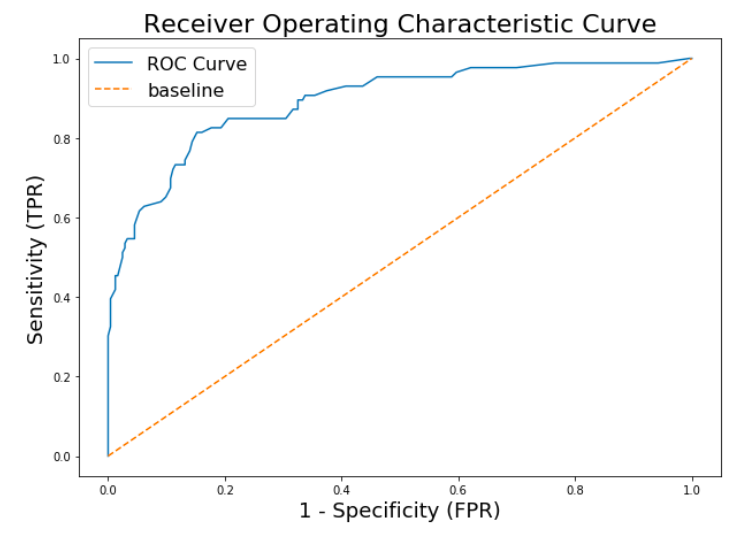
\includegraphics{Images/roc.png}

}

\caption{Model Performance on Test dataset}

\end{figure}

\hypertarget{model-stability-1}{%
\subsubsection{Model Stability}\label{model-stability-1}}

Following are model stability statistics: \textbf{Train vs.~Validation
dataset} 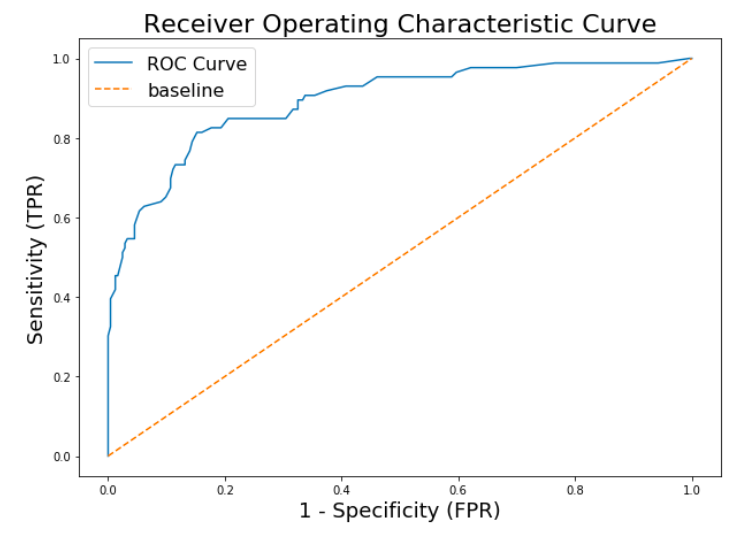
\includegraphics{Images/roc.png}

\textbf{Validation vs.~Test dataset} 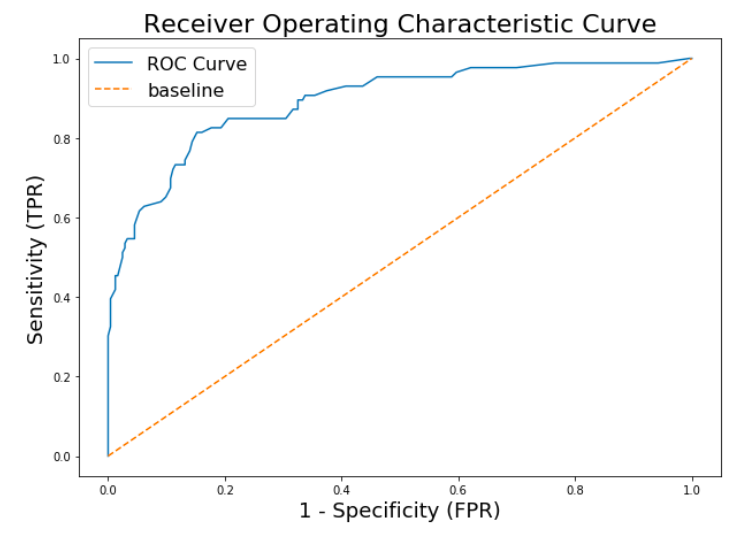
\includegraphics{Images/roc.png}

\hypertarget{model-performance-by-number-of-features}{%
\subsubsection{Model Performance by Number of
Features}\label{model-performance-by-number-of-features}}

Following is a summary of model performance, if it is replaced with a
model with subset of important features. This may be used to identify if
final model's performance maybe matched with a simpler model with less
number of features.



\end{document}
